\documentclass{article}
\usepackage[a3paper,landscape,margin=12mm]{geometry}
\usepackage[T1]{fontenc}
\usepackage[utf8]{inputenc}
\usepackage{tikz}
\usetikzlibrary{arrows.meta,positioning,calc}
\pagestyle{empty}

\definecolor{fpgaBlue}{RGB}{59,130,168}
\definecolor{controlFill}{RGB}{219,234,254}
\definecolor{clockFill}{RGB}{220,242,226}
\definecolor{alarmFill}{RGB}{254,232,218}
\definecolor{displayFill}{RGB}{252,239,204}
\definecolor{signalFill}{RGB}{226,236,246}
\definecolor{lineColor}{RGB}{71,85,105}

\tikzset{
  block/.style={draw, rounded corners=1pt, text width=3.7cm, minimum width=3.9cm,
    minimum height=1.7cm, align=center, font=\sffamily, text=black, line width=0.8pt},
  control/.style={block, fill=controlFill, minimum width=4cm},
  clock/.style={block, fill=clockFill},
  alarm/.style={block, fill=alarmFill, minimum width=4cm},
  display/.style={block, fill=displayFill, minimum width=3.8cm},
  signalbox/.style={block, fill=signalFill, minimum width=3.8cm},
  external/.style={draw, rounded corners=1pt, fill=white, text width=3.2cm,
    minimum width=3.4cm, minimum height=1.3cm, align=center, font=\sffamily,
    line width=0.7pt},
  signal/.style={-{Stealth[length=2.6mm]}, draw=lineColor, line width=0.8pt},
  label/.style={font=\sffamily\footnotesize, text width=2.4cm, align=center,
    fill=white, inner sep=1.5pt, text=black}
}

\begin{document}
\begin{center}
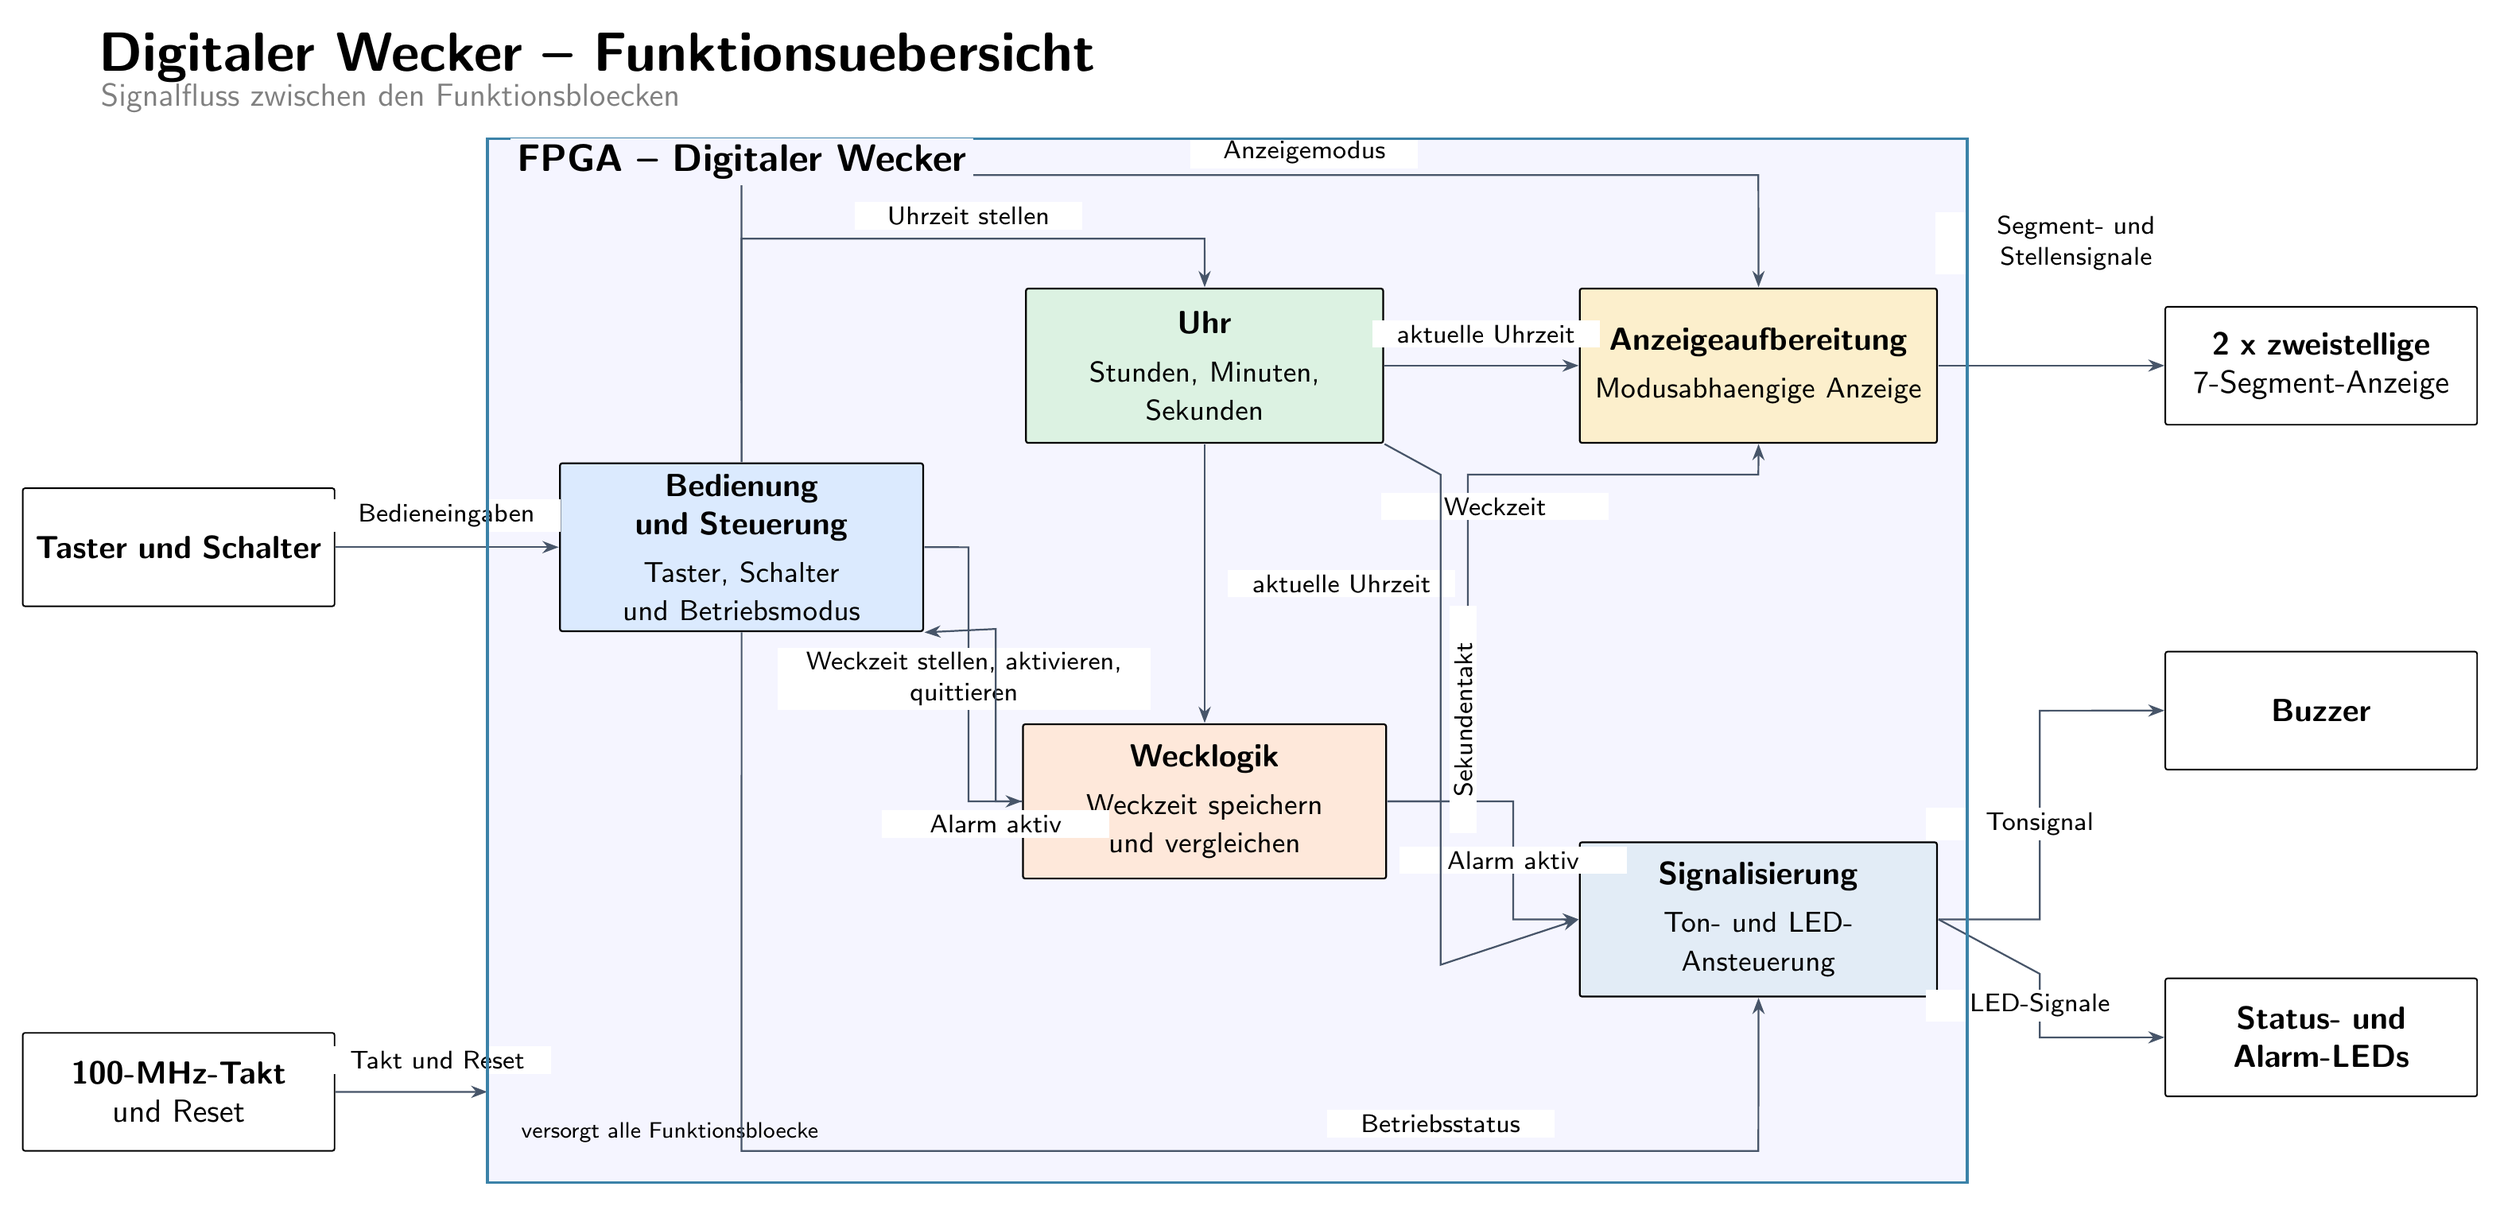
\begin{tikzpicture}[x=1cm,y=1cm,scale=1.45,transform shape]
  \node[anchor=west,font=\sffamily\bfseries\LARGE] at (-4.2,13.5)
    {Digitaler Wecker -- Funktionsuebersicht};
  \node[anchor=west,font=\sffamily\normalsize,text=gray] at (-4.18,13.05)
    {Signalfluss zwischen den Funktionsbloecken};

  \fill[blue!4] (0.2,1.1) rectangle (16.5,12.6);

  \node[control] (ctrl) at (3,8.1)
    {\textbf{Bedienung und Steuerung}\\[3pt]\small Taster, Schalter und Betriebsmodus};
  \node[clock] (clock) at (8.1,10.1)
    {\textbf{Uhr}\\[3pt]\small Stunden, Minuten, Sekunden};
  \node[alarm] (alarm) at (8.1,5.3)
    {\textbf{Wecklogik}\\[3pt]\small Weckzeit speichern und vergleichen};
  \node[display] (display) at (14.2,10.1)
    {\textbf{Anzeigeaufbereitung}\\[3pt]\small Modusabhaengige Anzeige};
  \node[signalbox] (signal) at (14.2,4)
    {\textbf{Signalisierung}\\[3pt]\small Ton- und LED-Ansteuerung};

  \node[external] (input) at (-3.2,8.1)
    {\textbf{Taster und Schalter}};
  \node[external] (clk) at (-3.2,2.1)
    {\textbf{100-MHz-Takt}\\und Reset};
  \node[external] (ssd) at (20.4,10.1)
    {\textbf{2 x zweistellige}\\7-Segment-Anzeige};
  \node[external] (buzzer) at (20.4,6.3)
    {\textbf{Buzzer}};
  \node[external] (led) at (20.4,2.7)
    {\textbf{Status- und Alarm-LEDs}};

  \draw[signal] (input.east) -- (ctrl.west);
  \node[label] at (-0.25,8.45) {Bedieneingaben};
  \draw[signal] (clk.east) -- (0.2,2.1);
  \node[label] at (-0.35,2.45) {Takt und Reset};
  \node[anchor=west,font=\sffamily\scriptsize] at (0.45,1.65)
    {versorgt alle Funktionsbloecke};
  \draw[signal] (ctrl.north) -- (3,11.5) -- (8.1,11.5) -- (clock.north);
  \node[label] at (5.5,11.75) {Uhrzeit stellen};
  \draw[signal] (ctrl.east) -- (5.5,8.1) -- (5.5,5.3) -- (alarm.west);
  \node[label,text width=4cm,align=center] at (5.45,6.65)
    {Weckzeit stellen, aktivieren,\\quittieren};
  \draw[signal] (clock.south) -- (alarm.north);
  \node[label,anchor=west] at (8.35,7.7) {aktuelle Uhrzeit};
  \draw[signal] (clock.east) -- (display.west);
  \node[label] at (11.2,10.45) {aktuelle Uhrzeit};
  \draw[signal] (alarm.east) -- (11,5.3) -- (11,8.9) -- (14.2,8.9) --
    (display.south);
  \node[label] at (11.3,8.55) {Weckzeit};
  \draw[signal] (ctrl.north) -- (3,12.2) -- (14.2,12.2) -- (display.north);
  \node[label] at (9.2,12.45) {Anzeigemodus};
  \draw[signal] (alarm.west) -- (5.8,5.3) -- (5.8,7.2) -- (ctrl.south east);
  \node[label] at (5.8,5.05) {Alarm aktiv};
  \draw[signal] (alarm.east) -- (11.5,5.3) -- (11.5,4) -- (signal.west);
  \node[label] at (11.5,4.65) {Alarm aktiv};
  \draw[signal] (ctrl.south) -- (3,1.45) -- (14.2,1.45) -- (signal.south);
  \node[label] at (10.7,1.75) {Betriebsstatus};
  \draw[signal] (clock.south east) -- (10.7,8.9) -- (10.7,3.5) -- (signal.west);
  \node[label,rotate=90] at (10.95,6.2) {Sekundentakt};
  \draw[signal] (display.east) -- (ssd.west);
  \node[label,text width=3cm] at (17.7,11.45) {Segment- und Stellensignale};
  \draw[signal] (signal.east) -- (17.3,4) -- (17.3,6.3) -- (buzzer.west);
  \node[label] at (17.3,5.05) {Tonsignal};
  \draw[signal] (signal.east) -- (17.3,3.4) -- (17.3,2.7) -- (led.west);
  \node[label] at (17.3,3.05) {LED-Signale};

  \draw[fpgaBlue,line width=1.2pt] (0.2,1.1) rectangle (16.5,12.6);
  \node[anchor=west,fill=blue!4,inner sep=2pt,font=\sffamily\bfseries\large]
    at (0.45,12.35) {FPGA -- Digitaler Wecker};
\end{tikzpicture}
\end{center}
\end{document}